\documentclass[1p]{elsarticle_modified}
%\bibliographystyle{elsarticle-num}

%\usepackage[colorlinks]{hyperref}
%\usepackage{abbrmath_seonhwa} %\Abb, \Ascr, \Acal ,\Abf, \Afrak
\usepackage{amsfonts}
\usepackage{amssymb}
\usepackage{amsmath}
\usepackage{amsthm}
\usepackage{scalefnt}
\usepackage{amsbsy}
\usepackage{kotex}
\usepackage{caption}
\usepackage{subfig}
\usepackage{color}
\usepackage{graphicx}
\usepackage{xcolor} %% white, black, red, green, blue, cyan, magenta, yellow
\usepackage{float}
\usepackage{setspace}
\usepackage{hyperref}

\usepackage{tikz}
\usetikzlibrary{arrows}

\usepackage{multirow}
\usepackage{array} % fixed length table
\usepackage{hhline}

%%%%%%%%%%%%%%%%%%%%%
\makeatletter
\renewcommand*\env@matrix[1][\arraystretch]{%
	\edef\arraystretch{#1}%
	\hskip -\arraycolsep
	\let\@ifnextchar\new@ifnextchar
	\array{*\c@MaxMatrixCols c}}
\makeatother %https://tex.stackexchange.com/questions/14071/how-can-i-increase-the-line-spacing-in-a-matrix
%%%%%%%%%%%%%%%

\usepackage[normalem]{ulem}

\newcommand{\msout}[1]{\ifmmode\text{\sout{\ensuremath{#1}}}\else\sout{#1}\fi}
%SOURCE: \msout is \stkout macro in https://tex.stackexchange.com/questions/20609/strikeout-in-math-mode

\newcommand{\cancel}[1]{
	\ifmmode
	{\color{red}\msout{#1}}
	\else
	{\color{red}\sout{#1}}
	\fi
}

\newcommand{\add}[1]{
	{\color{blue}\uwave{#1}}
}

\newcommand{\replace}[2]{
	\ifmmode
	{\color{red}\msout{#1}}{\color{blue}\uwave{#2}}
	\else
	{\color{red}\sout{#1}}{\color{blue}\uwave{#2}}
	\fi
}

\newcommand{\Sol}{\mathcal{S}} %segment
\newcommand{\D}{D} %diagram
\newcommand{\A}{\mathcal{A}} %arc


%%%%%%%%%%%%%%%%%%%%%%%%%%%%%5 test

\def\sl{\operatorname{\textup{SL}}(2,\Cbb)}
\def\psl{\operatorname{\textup{PSL}}(2,\Cbb)}
\def\quan{\mkern 1mu \triangleright \mkern 1mu}

\theoremstyle{definition}
\newtheorem{thm}{Theorem}[section]
\newtheorem{prop}[thm]{Proposition}
\newtheorem{lem}[thm]{Lemma}
\newtheorem{ques}[thm]{Question}
\newtheorem{cor}[thm]{Corollary}
\newtheorem{defn}[thm]{Definition}
\newtheorem{exam}[thm]{Example}
\newtheorem{rmk}[thm]{Remark}
\newtheorem{alg}[thm]{Algorithm}

\newcommand{\I}{\sqrt{-1}}
\begin{document}

%\begin{frontmatter}
%
%\title{Boundary parabolic representations of knots up to 8 crossings}
%
%%% Group authors per affiliation:
%\author{Yunhi Cho} 
%\address{Department of Mathematics, University of Seoul, Seoul, Korea}
%\ead{yhcho@uos.ac.kr}
%
%
%\author{Seonhwa Kim} %\fnref{s_kim}}
%\address{Center for Geometry and Physics, Institute for Basic Science, Pohang, 37673, Korea}
%\ead{ryeona17@ibs.re.kr}
%
%\author{Hyuk Kim}
%\address{Department of Mathematical Sciences, Seoul National University, Seoul 08826, Korea}
%\ead{hyukkim@snu.ac.kr}
%
%\author{Seokbeom Yoon}
%\address{Department of Mathematical Sciences, Seoul National University, Seoul, 08826,  Korea}
%\ead{sbyoon15@snu.ac.kr}
%
%\begin{abstract}
%We find all boundary parabolic representation of knots up to 8 crossings.
%
%\end{abstract}
%\begin{keyword}
%    \MSC[2010] 57M25 
%\end{keyword}
%
%\end{frontmatter}

%\linenumbers
%\tableofcontents
%
\newcommand\colored[1]{\textcolor{white}{\rule[-0.35ex]{0.8em}{1.4ex}}\kern-0.8em\color{red} #1}%
%\newcommand\colored[1]{\textcolor{white}{ #1}\kern-2.17ex	\textcolor{white}{ #1}\kern-1.81ex	\textcolor{white}{ #1}\kern-2.15ex\color{red}#1	}

{\Large $\underline{12a_{0540}~(K12a_{0540})}$}

\setlength{\tabcolsep}{10pt}
\renewcommand{\arraystretch}{1.6}
\vspace{1cm}\begin{tabular}{m{100pt}>{\centering\arraybackslash}m{274pt}}
\multirow{5}{120pt}{
	\centering
	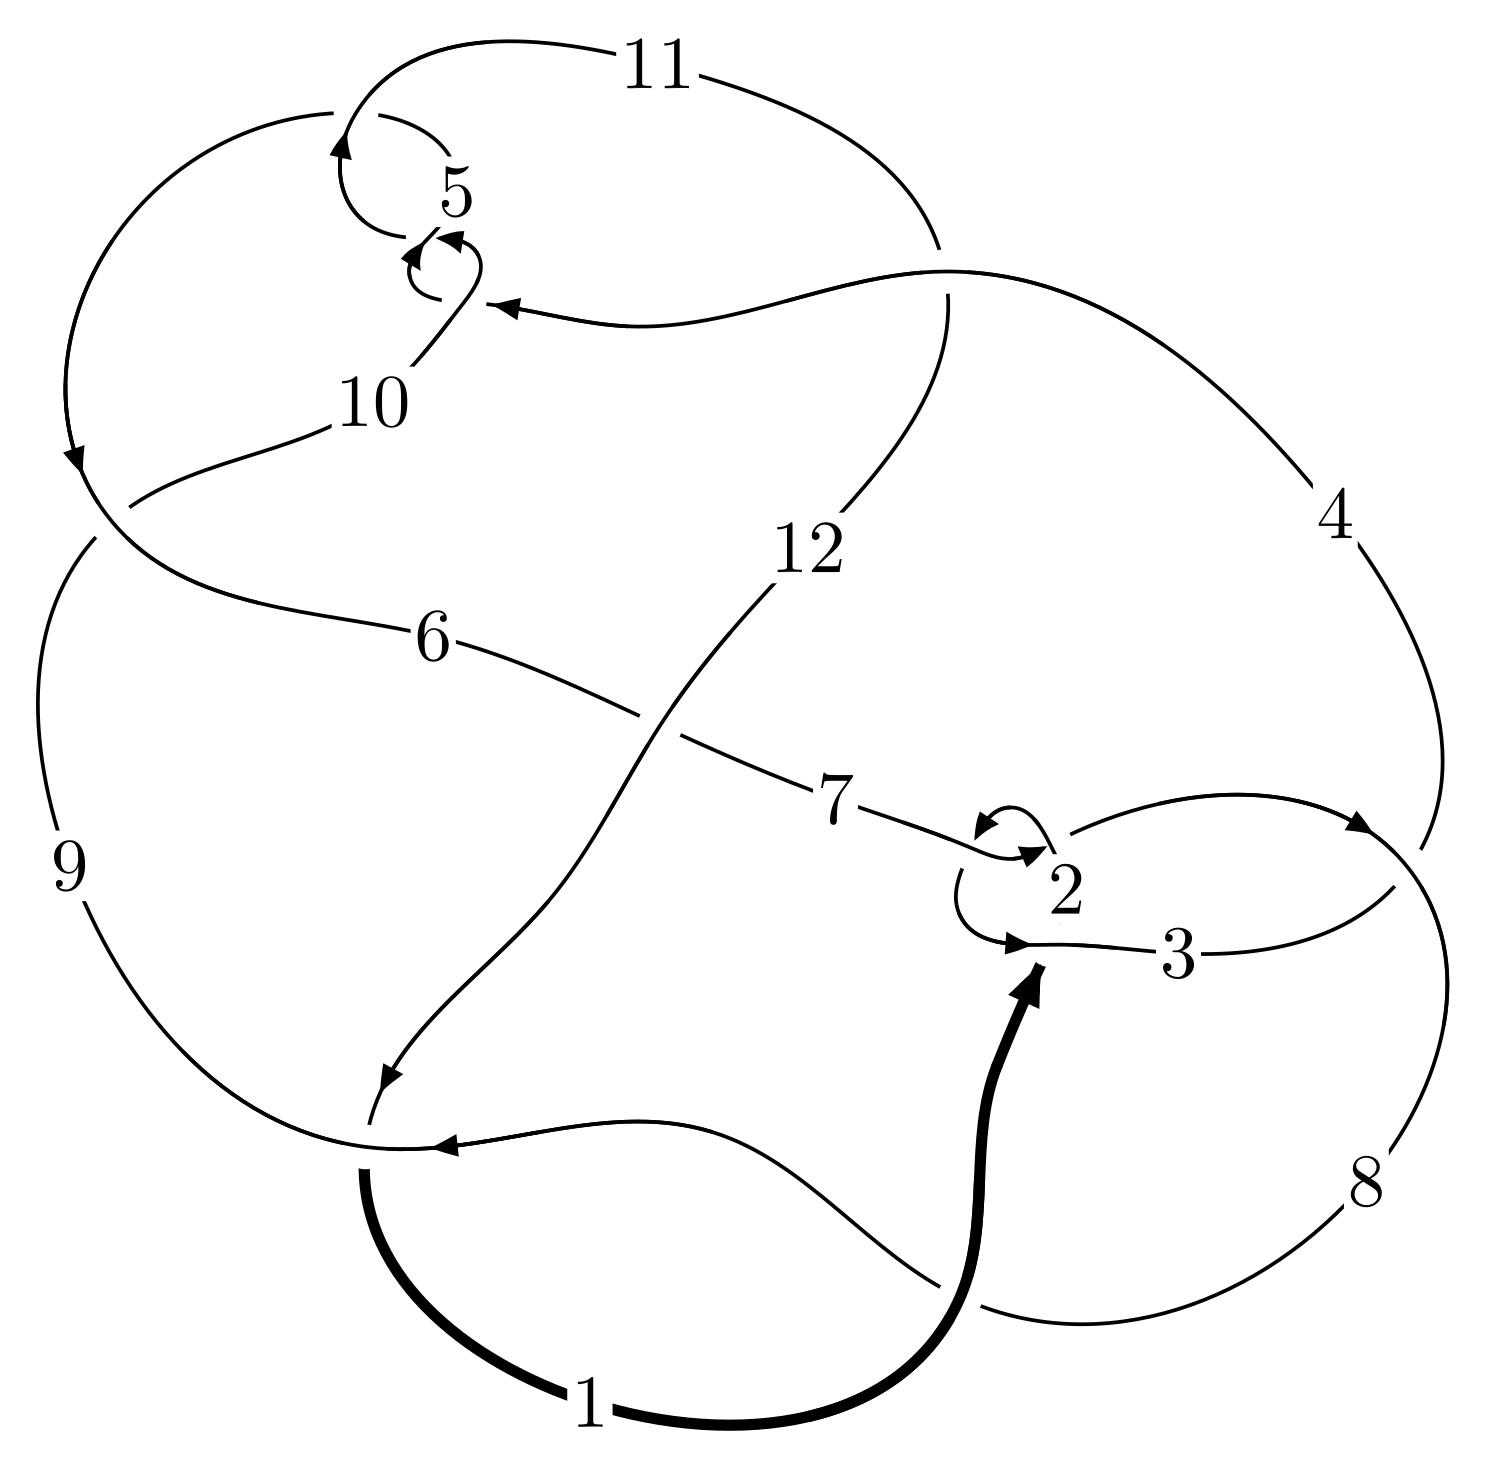
\includegraphics[width=112pt]{../../../GIT/diagram.site/Diagrams/png/1341_12a_0540.png}\\
\ \ \ A knot diagram\footnotemark}&
\allowdisplaybreaks
\textbf{Linearized knot diagam} \\
\cline{2-2}
 &
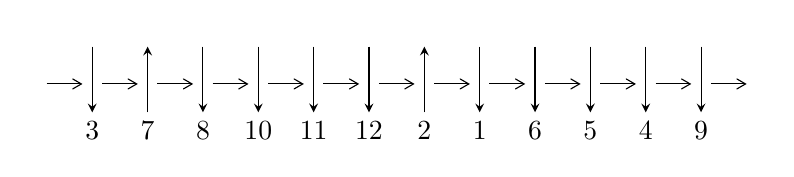
\begin{tikzpicture}[x=20pt, y=17pt]
	% nodes
	\node (C0) at (0, 0) {};
	\node (C1) at (1, 0) {};
	\node (C1U) at (1, +1) {};
	\node (C1D) at (1, -1) {3};

	\node (C2) at (2, 0) {};
	\node (C2U) at (2, +1) {};
	\node (C2D) at (2, -1) {7};

	\node (C3) at (3, 0) {};
	\node (C3U) at (3, +1) {};
	\node (C3D) at (3, -1) {8};

	\node (C4) at (4, 0) {};
	\node (C4U) at (4, +1) {};
	\node (C4D) at (4, -1) {10};

	\node (C5) at (5, 0) {};
	\node (C5U) at (5, +1) {};
	\node (C5D) at (5, -1) {11};

	\node (C6) at (6, 0) {};
	\node (C6U) at (6, +1) {};
	\node (C6D) at (6, -1) {12};

	\node (C7) at (7, 0) {};
	\node (C7U) at (7, +1) {};
	\node (C7D) at (7, -1) {2};

	\node (C8) at (8, 0) {};
	\node (C8U) at (8, +1) {};
	\node (C8D) at (8, -1) {1};

	\node (C9) at (9, 0) {};
	\node (C9U) at (9, +1) {};
	\node (C9D) at (9, -1) {6};

	\node (C10) at (10, 0) {};
	\node (C10U) at (10, +1) {};
	\node (C10D) at (10, -1) {5};

	\node (C11) at (11, 0) {};
	\node (C11U) at (11, +1) {};
	\node (C11D) at (11, -1) {4};

	\node (C12) at (12, 0) {};
	\node (C12U) at (12, +1) {};
	\node (C12D) at (12, -1) {9};
	\node (C13) at (13, 0) {};

	% arrows
	\draw[->,>={angle 60}]
	(C0) edge (C1) (C1) edge (C2) (C2) edge (C3) (C3) edge (C4) (C4) edge (C5) (C5) edge (C6) (C6) edge (C7) (C7) edge (C8) (C8) edge (C9) (C9) edge (C10) (C10) edge (C11) (C11) edge (C12) (C12) edge (C13) ;	\draw[->,>=stealth]
	(C1U) edge (C1D) (C2D) edge (C2U) (C3U) edge (C3D) (C4U) edge (C4D) (C5U) edge (C5D) (C6U) edge (C6D) (C7D) edge (C7U) (C8U) edge (C8D) (C9U) edge (C9D) (C10U) edge (C10D) (C11U) edge (C11D) (C12U) edge (C12D) ;
	\end{tikzpicture} \\
\hhline{~~} \\& 
\textbf{Solving Sequence} \\ \cline{2-2} 
 &
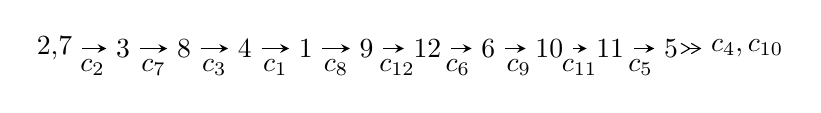
\begin{tikzpicture}[x=22pt, y=7pt]
	% node
	\node (A0) at (-1/8, 0) {2,7};
	\node (A1) at (1, 0) {3};
	\node (A2) at (2, 0) {8};
	\node (A3) at (3, 0) {4};
	\node (A4) at (4, 0) {1};
	\node (A5) at (5, 0) {9};
	\node (A6) at (6, 0) {12};
	\node (A7) at (7, 0) {6};
	\node (A8) at (8, 0) {10};
	\node (A9) at (9, 0) {11};
	\node (A10) at (10, 0) {5};
	\node (C1) at (1/2, -1) {$c_{2}$};
	\node (C2) at (3/2, -1) {$c_{7}$};
	\node (C3) at (5/2, -1) {$c_{3}$};
	\node (C4) at (7/2, -1) {$c_{1}$};
	\node (C5) at (9/2, -1) {$c_{8}$};
	\node (C6) at (11/2, -1) {$c_{12}$};
	\node (C7) at (13/2, -1) {$c_{6}$};
	\node (C8) at (15/2, -1) {$c_{9}$};
	\node (C9) at (17/2, -1) {$c_{11}$};
	\node (C10) at (19/2, -1) {$c_{5}$};
	\node (A11) at (45/4, 0) {$c_{4},c_{10}$};

	% edge
	\draw[->,>=stealth]	
	(A0) edge (A1) (A1) edge (A2) (A2) edge (A3) (A3) edge (A4) (A4) edge (A5) (A5) edge (A6) (A6) edge (A7) (A7) edge (A8) (A8) edge (A9) (A9) edge (A10) ;
	\draw[->>,>={angle 60}]	
	(A10) edge (A11);
\end{tikzpicture} \\ 

\end{tabular} \\

\footnotetext{
The image of knot diagram is generated by the software ``\textbf{Draw programme}" developed by Andrew Bartholomew(\url{http://www.layer8.co.uk/maths/draw/index.htm\#Running-draw}), where we modified some parts for our purpose(\url{https://github.com/CATsTAILs/LinksPainter}).
}\phantom \\ \newline 
\centering \textbf{Ideals for irreducible components\footnotemark of $X_{\text{par}}$} 
 
\begin{align*}
I^u_{1}&=\langle 
u^{82}- u^{81}+\cdots+3 u-1\rangle \\
\\
\end{align*}
\raggedright * 1 irreducible components of $\dim_{\mathbb{C}}=0$, with total 82 representations.\\
\footnotetext{All coefficients of polynomials are rational numbers. But the coefficients are sometimes approximated in decimal forms when there is not enough margin.}
\newpage
\renewcommand{\arraystretch}{1}
\centering \section*{I. $I^u_{1}= \langle u^{82}- u^{81}+\cdots+3 u-1 \rangle$}
\flushleft \textbf{(i) Arc colorings}\\
\begin{tabular}{m{7pt} m{180pt} m{7pt} m{180pt} }
\flushright $a_{2}=$&$\begin{pmatrix}1\\0\end{pmatrix}$ \\
\flushright $a_{7}=$&$\begin{pmatrix}0\\u\end{pmatrix}$ \\
\flushright $a_{3}=$&$\begin{pmatrix}1\\- u^2\end{pmatrix}$ \\
\flushright $a_{8}=$&$\begin{pmatrix}u\\u\end{pmatrix}$ \\
\flushright $a_{4}=$&$\begin{pmatrix}u^4+u^2+1\\u^4\end{pmatrix}$ \\
\flushright $a_{1}=$&$\begin{pmatrix}u^2+1\\- u^4\end{pmatrix}$ \\
\flushright $a_{9}=$&$\begin{pmatrix}- u^7-2 u^5-2 u^3\\u^9+u^7+u^5+u\end{pmatrix}$ \\
\flushright $a_{12}=$&$\begin{pmatrix}u^{12}+3 u^{10}+5 u^8+4 u^6+2 u^4+u^2+1\\- u^{14}-2 u^{12}-3 u^{10}-2 u^8-2 u^6-2 u^4- u^2\end{pmatrix}$ \\
\flushright $a_{6}=$&$\begin{pmatrix}u^{25}+6 u^{23}+\cdots+2 u^3+u\\- u^{27}-5 u^{25}+\cdots- u^3+u\end{pmatrix}$ \\
\flushright $a_{10}=$&$\begin{pmatrix}- u^{43}-10 u^{41}+\cdots-8 u^5-3 u^3\\u^{45}+9 u^{43}+\cdots- u^3+u\end{pmatrix}$ \\
\flushright $a_{11}=$&$\begin{pmatrix}- u^{22}-5 u^{20}+\cdots-3 u^4+1\\- u^{22}-4 u^{20}+\cdots-2 u^4- u^2\end{pmatrix}$ \\
\flushright $a_{5}=$&$\begin{pmatrix}- u^{71}-16 u^{69}+\cdots+2 u^3+2 u\\- u^{71}-15 u^{69}+\cdots-2 u^3+u\end{pmatrix}$\\&\end{tabular}
\flushleft \textbf{(ii) Obstruction class $= -1$}\\~\\
\flushleft \textbf{(iii) Cusp Shapes $= 4 u^{80}-4 u^{79}+\cdots+16 u-18$}\\~\\
\newpage\renewcommand{\arraystretch}{1}
\flushleft \textbf{(iv) u-Polynomials at the component}\newline \\
\begin{tabular}{m{50pt}|m{274pt}}
Crossings & \hspace{64pt}u-Polynomials at each crossing \\
\hline $$\begin{aligned}c_{1}\end{aligned}$$&$\begin{aligned}
&u^{82}+37 u^{81}+\cdots-3 u+1
\end{aligned}$\\
\hline $$\begin{aligned}c_{2},c_{7}\end{aligned}$$&$\begin{aligned}
&u^{82}+u^{81}+\cdots-3 u-1
\end{aligned}$\\
\hline $$\begin{aligned}c_{3}\end{aligned}$$&$\begin{aligned}
&u^{82}- u^{81}+\cdots+13 u-2
\end{aligned}$\\
\hline $$\begin{aligned}c_{4},c_{5},c_{10}\end{aligned}$$&$\begin{aligned}
&u^{82}- u^{81}+\cdots-3 u-1
\end{aligned}$\\
\hline $$\begin{aligned}c_{6}\end{aligned}$$&$\begin{aligned}
&u^{82}+u^{81}+\cdots-1107 u-521
\end{aligned}$\\
\hline $$\begin{aligned}c_{8},c_{12}\end{aligned}$$&$\begin{aligned}
&u^{82}+5 u^{81}+\cdots-208 u-16
\end{aligned}$\\
\hline $$\begin{aligned}c_{9},c_{11}\end{aligned}$$&$\begin{aligned}
&u^{82}+3 u^{81}+\cdots+503 u+88
\end{aligned}$\\
\hline
\end{tabular}\\~\\
\newpage\renewcommand{\arraystretch}{1}
\flushleft \textbf{(v) Riley Polynomials at the component}\newline \\
\begin{tabular}{m{50pt}|m{274pt}}
Crossings & \hspace{64pt}Riley Polynomials at each crossing \\
\hline $$\begin{aligned}c_{1}\end{aligned}$$&$\begin{aligned}
&y^{82}+17 y^{81}+\cdots-31 y+1
\end{aligned}$\\
\hline $$\begin{aligned}c_{2},c_{7}\end{aligned}$$&$\begin{aligned}
&y^{82}+37 y^{81}+\cdots-3 y+1
\end{aligned}$\\
\hline $$\begin{aligned}c_{3}\end{aligned}$$&$\begin{aligned}
&y^{82}-3 y^{81}+\cdots-281 y+4
\end{aligned}$\\
\hline $$\begin{aligned}c_{4},c_{5},c_{10}\end{aligned}$$&$\begin{aligned}
&y^{82}-67 y^{81}+\cdots-3 y+1
\end{aligned}$\\
\hline $$\begin{aligned}c_{6}\end{aligned}$$&$\begin{aligned}
&y^{82}+17 y^{81}+\cdots+5469401 y+271441
\end{aligned}$\\
\hline $$\begin{aligned}c_{8},c_{12}\end{aligned}$$&$\begin{aligned}
&y^{82}+65 y^{81}+\cdots-5920 y+256
\end{aligned}$\\
\hline $$\begin{aligned}c_{9},c_{11}\end{aligned}$$&$\begin{aligned}
&y^{82}+57 y^{81}+\cdots-88625 y+7744
\end{aligned}$\\
\hline
\end{tabular}\\~\\
\newpage\flushleft \textbf{(vi) Complex Volumes and Cusp Shapes}
$$\begin{array}{c|c|c}  
\text{Solutions to }I^u_{1}& \I (\text{vol} + \sqrt{-1}CS) & \text{Cusp shape}\\
 \hline 
\begin{aligned}
u &= \phantom{-}0.133466 + 1.000640 I\end{aligned}
 & -1.27367 - 1.16757 I & \phantom{-0.000000 } 0 \\ \hline\begin{aligned}
u &= \phantom{-}0.133466 - 1.000640 I\end{aligned}
 & -1.27367 + 1.16757 I & \phantom{-0.000000 } 0 \\ \hline\begin{aligned}
u &= -0.532862 + 0.830572 I\end{aligned}
 & -0.02430 - 6.14834 I & \phantom{-0.000000 } 0 \\ \hline\begin{aligned}
u &= -0.532862 - 0.830572 I\end{aligned}
 & -0.02430 + 6.14834 I & \phantom{-0.000000 } 0 \\ \hline\begin{aligned}
u &= \phantom{-}0.524056 + 0.795819 I\end{aligned}
 & \phantom{-}4.00847 + 2.15498 I & \phantom{-0.000000 } 0. - 3.78589 I \\ \hline\begin{aligned}
u &= \phantom{-}0.524056 - 0.795819 I\end{aligned}
 & \phantom{-}4.00847 - 2.15498 I & \phantom{-0.000000 -}0. + 3.78589 I \\ \hline\begin{aligned}
u &= -0.284834 + 0.897551 I\end{aligned}
 & -0.67768 - 1.28884 I & -8.00000 + 4.92802 I \\ \hline\begin{aligned}
u &= -0.284834 - 0.897551 I\end{aligned}
 & -0.67768 + 1.28884 I & -8.00000 - 4.92802 I \\ \hline\begin{aligned}
u &= -0.170246 + 1.062460 I\end{aligned}
 & -6.83445 + 2.33727 I & \phantom{-0.000000 } 0 \\ \hline\begin{aligned}
u &= -0.170246 - 1.062460 I\end{aligned}
 & -6.83445 - 2.33727 I & \phantom{-0.000000 } 0 \\ \hline\begin{aligned}
u &= -0.749314 + 0.538316 I\end{aligned}
 & \phantom{-}4.42162 - 7.61184 I & -4.45987 + 5.77896 I \\ \hline\begin{aligned}
u &= -0.749314 - 0.538316 I\end{aligned}
 & \phantom{-}4.42162 + 7.61184 I & -4.45987 - 5.77896 I \\ \hline\begin{aligned}
u &= \phantom{-}0.752586 + 0.529461 I\end{aligned}
 & \phantom{-}8.86798 + 3.35426 I & \phantom{-0.000000 } 0. - 3.38737 I \\ \hline\begin{aligned}
u &= \phantom{-}0.752586 - 0.529461 I\end{aligned}
 & \phantom{-}8.86798 - 3.35426 I & \phantom{-0.000000 -}0. + 3.38737 I \\ \hline\begin{aligned}
u &= -0.525332 + 0.751819 I\end{aligned}
 & \phantom{-}0.19898 + 1.80626 I & -5.15609 + 0. I\phantom{ +0.000000I} \\ \hline\begin{aligned}
u &= -0.525332 - 0.751819 I\end{aligned}
 & \phantom{-}0.19898 - 1.80626 I & -5.15609 + 0. I\phantom{ +0.000000I} \\ \hline\begin{aligned}
u &= -0.755993 + 0.517707 I\end{aligned}
 & \phantom{-}5.56056 + 0.94896 I & -3.15680 + 0. I\phantom{ +0.000000I} \\ \hline\begin{aligned}
u &= -0.755993 - 0.517707 I\end{aligned}
 & \phantom{-}5.56056 - 0.94896 I & -3.15680 + 0. I\phantom{ +0.000000I} \\ \hline\begin{aligned}
u &= \phantom{-}0.287923 + 1.044900 I\end{aligned}
 & -4.82508 + 3.82270 I & \phantom{-0.000000 } 0 \\ \hline\begin{aligned}
u &= \phantom{-}0.287923 - 1.044900 I\end{aligned}
 & -4.82508 - 3.82270 I & \phantom{-0.000000 } 0 \\ \hline\begin{aligned}
u &= \phantom{-}0.081808 + 1.082030 I\end{aligned}
 & -0.0248733 - 0.0847749 I & \phantom{-0.000000 } 0 \\ \hline\begin{aligned}
u &= \phantom{-}0.081808 - 1.082030 I\end{aligned}
 & -0.0248733 + 0.0847749 I & \phantom{-0.000000 } 0 \\ \hline\begin{aligned}
u &= -0.098958 + 1.094980 I\end{aligned}
 & \phantom{-}3.18345 + 4.26960 I & \phantom{-0.000000 } 0 \\ \hline\begin{aligned}
u &= -0.098958 - 1.094980 I\end{aligned}
 & \phantom{-}3.18345 - 4.26960 I & \phantom{-0.000000 } 0 \\ \hline\begin{aligned}
u &= \phantom{-}0.781133 + 0.445371 I\end{aligned}
 & \phantom{-}5.16257 - 1.98343 I & -3.74120 + 0. I\phantom{ +0.000000I} \\ \hline\begin{aligned}
u &= \phantom{-}0.781133 - 0.445371 I\end{aligned}
 & \phantom{-}5.16257 + 1.98343 I & -3.74120 + 0. I\phantom{ +0.000000I} \\ \hline\begin{aligned}
u &= -0.785449 + 0.435883 I\end{aligned}
 & \phantom{-}8.35181 + 6.28657 I & -0.78678 - 3.84368 I \\ \hline\begin{aligned}
u &= -0.785449 - 0.435883 I\end{aligned}
 & \phantom{-}8.35181 - 6.28657 I & -0.78678 + 3.84368 I \\ \hline\begin{aligned}
u &= \phantom{-}0.787695 + 0.428827 I\end{aligned}
 & \phantom{-}3.81832 - 10.53440 I & -5.33981 + 6.01257 I \\ \hline\begin{aligned}
u &= \phantom{-}0.787695 - 0.428827 I\end{aligned}
 & \phantom{-}3.81832 + 10.53440 I & -5.33981 - 6.01257 I\\
 \hline 
 \end{array}$$\newpage$$\begin{array}{c|c|c}  
\text{Solutions to }I^u_{1}& \I (\text{vol} + \sqrt{-1}CS) & \text{Cusp shape}\\
 \hline 
\begin{aligned}
u &= \phantom{-}0.109809 + 1.102990 I\end{aligned}
 & -1.33118 - 8.43930 I & \phantom{-0.000000 } 0 \\ \hline\begin{aligned}
u &= \phantom{-}0.109809 - 1.102990 I\end{aligned}
 & -1.33118 + 8.43930 I & \phantom{-0.000000 } 0 \\ \hline\begin{aligned}
u &= -0.359135 + 1.056470 I\end{aligned}
 & -1.102440 - 0.747841 I & \phantom{-0.000000 } 0 \\ \hline\begin{aligned}
u &= -0.359135 - 1.056470 I\end{aligned}
 & -1.102440 + 0.747841 I & \phantom{-0.000000 } 0 \\ \hline\begin{aligned}
u &= -0.724858 + 0.480472 I\end{aligned}
 & \phantom{-}3.67849 - 0.28703 I & -3.38751 + 3.80148 I \\ \hline\begin{aligned}
u &= -0.724858 - 0.480472 I\end{aligned}
 & \phantom{-}3.67849 + 0.28703 I & -3.38751 - 3.80148 I \\ \hline\begin{aligned}
u &= \phantom{-}0.743794 + 0.448446 I\end{aligned}
 & \phantom{-}3.49632 - 2.84575 I & -4.21837 + 4.55562 I \\ \hline\begin{aligned}
u &= \phantom{-}0.743794 - 0.448446 I\end{aligned}
 & \phantom{-}3.49632 + 2.84575 I & -4.21837 - 4.55562 I \\ \hline\begin{aligned}
u &= \phantom{-}0.430453 + 1.053190 I\end{aligned}
 & -3.25125 + 3.38062 I & \phantom{-0.000000 } 0 \\ \hline\begin{aligned}
u &= \phantom{-}0.430453 - 1.053190 I\end{aligned}
 & -3.25125 - 3.38062 I & \phantom{-0.000000 } 0 \\ \hline\begin{aligned}
u &= \phantom{-}0.365552 + 1.084130 I\end{aligned}
 & -5.57182 - 2.81011 I & \phantom{-0.000000 } 0 \\ \hline\begin{aligned}
u &= \phantom{-}0.365552 - 1.084130 I\end{aligned}
 & -5.57182 + 2.81011 I & \phantom{-0.000000 } 0 \\ \hline\begin{aligned}
u &= -0.744053 + 0.414739 I\end{aligned}
 & -2.14948 + 4.40174 I & -9.50950 - 3.74202 I \\ \hline\begin{aligned}
u &= -0.744053 - 0.414739 I\end{aligned}
 & -2.14948 - 4.40174 I & -9.50950 + 3.74202 I \\ \hline\begin{aligned}
u &= \phantom{-}0.679349 + 0.510566 I\end{aligned}
 & -1.62052 + 2.05298 I & -8.39395 - 3.31884 I \\ \hline\begin{aligned}
u &= \phantom{-}0.679349 - 0.510566 I\end{aligned}
 & -1.62052 - 2.05298 I & -8.39395 + 3.31884 I \\ \hline\begin{aligned}
u &= \phantom{-}0.495189 + 1.047400 I\end{aligned}
 & -3.38134 + 2.83643 I & \phantom{-0.000000 } 0 \\ \hline\begin{aligned}
u &= \phantom{-}0.495189 - 1.047400 I\end{aligned}
 & -3.38134 - 2.83643 I & \phantom{-0.000000 } 0 \\ \hline\begin{aligned}
u &= -0.423498 + 1.091700 I\end{aligned}
 & -9.08228 - 3.64788 I & \phantom{-0.000000 } 0 \\ \hline\begin{aligned}
u &= -0.423498 - 1.091700 I\end{aligned}
 & -9.08228 + 3.64788 I & \phantom{-0.000000 } 0 \\ \hline\begin{aligned}
u &= -0.475657 + 1.085560 I\end{aligned}
 & -0.31884 - 6.30832 I & \phantom{-0.000000 } 0 \\ \hline\begin{aligned}
u &= -0.475657 - 1.085560 I\end{aligned}
 & -0.31884 + 6.30832 I & \phantom{-0.000000 } 0 \\ \hline\begin{aligned}
u &= \phantom{-}0.563996 + 1.045740 I\end{aligned}
 & -3.20812 + 2.76694 I & \phantom{-0.000000 } 0 \\ \hline\begin{aligned}
u &= \phantom{-}0.563996 - 1.045740 I\end{aligned}
 & -3.20812 - 2.76694 I & \phantom{-0.000000 } 0 \\ \hline\begin{aligned}
u &= \phantom{-}0.470135 + 1.098680 I\end{aligned}
 & -4.87213 + 10.11490 I & \phantom{-0.000000 } 0 \\ \hline\begin{aligned}
u &= \phantom{-}0.470135 - 1.098680 I\end{aligned}
 & -4.87213 - 10.11490 I & \phantom{-0.000000 } 0 \\ \hline\begin{aligned}
u &= -0.620596 + 1.036150 I\end{aligned}
 & \phantom{-}2.94040 + 2.41061 I & \phantom{-0.000000 } 0 \\ \hline\begin{aligned}
u &= -0.620596 - 1.036150 I\end{aligned}
 & \phantom{-}2.94040 - 2.41061 I & \phantom{-0.000000 } 0 \\ \hline\begin{aligned}
u &= \phantom{-}0.620020 + 1.042550 I\end{aligned}
 & \phantom{-}7.34120 + 1.85374 I & \phantom{-0.000000 } 0 \\ \hline\begin{aligned}
u &= \phantom{-}0.620020 - 1.042550 I\end{aligned}
 & \phantom{-}7.34120 - 1.85374 I & \phantom{-0.000000 } 0\\
 \hline 
 \end{array}$$\newpage$$\begin{array}{c|c|c}  
\text{Solutions to }I^u_{1}& \I (\text{vol} + \sqrt{-1}CS) & \text{Cusp shape}\\
 \hline 
\begin{aligned}
u &= -0.592434 + 1.063710 I\end{aligned}
 & \phantom{-}1.94954 - 4.75248 I & \phantom{-0.000000 } 0 \\ \hline\begin{aligned}
u &= -0.592434 - 1.063710 I\end{aligned}
 & \phantom{-}1.94954 + 4.75248 I & \phantom{-0.000000 } 0 \\ \hline\begin{aligned}
u &= -0.618735 + 1.050250 I\end{aligned}
 & \phantom{-}3.97605 - 6.16137 I & \phantom{-0.000000 } 0 \\ \hline\begin{aligned}
u &= -0.618735 - 1.050250 I\end{aligned}
 & \phantom{-}3.97605 + 6.16137 I & \phantom{-0.000000 } 0 \\ \hline\begin{aligned}
u &= \phantom{-}0.595132 + 1.081620 I\end{aligned}
 & \phantom{-}1.62331 + 7.94105 I & \phantom{-0.000000 } 0 \\ \hline\begin{aligned}
u &= \phantom{-}0.595132 - 1.081620 I\end{aligned}
 & \phantom{-}1.62331 - 7.94105 I & \phantom{-0.000000 } 0 \\ \hline\begin{aligned}
u &= -0.587329 + 1.094110 I\end{aligned}
 & -4.15024 - 9.46471 I & \phantom{-0.000000 } 0 \\ \hline\begin{aligned}
u &= -0.587329 - 1.094110 I\end{aligned}
 & -4.15024 + 9.46471 I & \phantom{-0.000000 } 0 \\ \hline\begin{aligned}
u &= \phantom{-}0.609197 + 1.092830 I\end{aligned}
 & \phantom{-}3.23683 + 7.22327 I & \phantom{-0.000000 } 0 \\ \hline\begin{aligned}
u &= \phantom{-}0.609197 - 1.092830 I\end{aligned}
 & \phantom{-}3.23683 - 7.22327 I & \phantom{-0.000000 } 0 \\ \hline\begin{aligned}
u &= -0.608118 + 1.098090 I\end{aligned}
 & \phantom{-}6.38214 - 11.53260 I & \phantom{-0.000000 } 0 \\ \hline\begin{aligned}
u &= -0.608118 - 1.098090 I\end{aligned}
 & \phantom{-}6.38214 + 11.53260 I & \phantom{-0.000000 } 0 \\ \hline\begin{aligned}
u &= \phantom{-}0.606813 + 1.101570 I\end{aligned}
 & \phantom{-}1.8176 + 15.7804 I & \phantom{-0.000000 } 0 \\ \hline\begin{aligned}
u &= \phantom{-}0.606813 - 1.101570 I\end{aligned}
 & \phantom{-}1.8176 - 15.7804 I & \phantom{-0.000000 } 0 \\ \hline\begin{aligned}
u &= \phantom{-}0.567507 + 0.269437 I\end{aligned}
 & -1.29725 + 1.34677 I & -7.56967 - 0.28082 I \\ \hline\begin{aligned}
u &= \phantom{-}0.567507 - 0.269437 I\end{aligned}
 & -1.29725 - 1.34677 I & -7.56967 + 0.28082 I \\ \hline\begin{aligned}
u &= \phantom{-}0.609013 + 0.145464 I\end{aligned}
 & -2.26753 - 6.00853 I & -9.43299 + 5.77985 I \\ \hline\begin{aligned}
u &= \phantom{-}0.609013 - 0.145464 I\end{aligned}
 & -2.26753 + 6.00853 I & -9.43299 - 5.77985 I \\ \hline\begin{aligned}
u &= -0.581311 + 0.180322 I\end{aligned}
 & \phantom{-}2.13139 + 2.21650 I & -4.07689 - 3.88447 I \\ \hline\begin{aligned}
u &= -0.581311 - 0.180322 I\end{aligned}
 & \phantom{-}2.13139 - 2.21650 I & -4.07689 + 3.88447 I \\ \hline\begin{aligned}
u &= -0.572870\phantom{ +0.000000I}\end{aligned}
 & -6.20998\phantom{ +0.000000I} & -14.2450\phantom{ +0.000000I} \\ \hline\begin{aligned}
u &= \phantom{-}0.421035\phantom{ +0.000000I}\end{aligned}
 & -0.786796\phantom{ +0.000000I} & -12.6530\phantom{ +0.000000I}\\
 \hline 
 \end{array}$$\newpage
\newpage\renewcommand{\arraystretch}{1}
\centering \section*{ II. u-Polynomials}
\begin{tabular}{m{50pt}|m{274pt}}
Crossings & \hspace{64pt}u-Polynomials at each crossing \\
\hline $$\begin{aligned}c_{1}\end{aligned}$$&$\begin{aligned}
&u^{82}+37 u^{81}+\cdots-3 u+1
\end{aligned}$\\
\hline $$\begin{aligned}c_{2},c_{7}\end{aligned}$$&$\begin{aligned}
&u^{82}+u^{81}+\cdots-3 u-1
\end{aligned}$\\
\hline $$\begin{aligned}c_{3}\end{aligned}$$&$\begin{aligned}
&u^{82}- u^{81}+\cdots+13 u-2
\end{aligned}$\\
\hline $$\begin{aligned}c_{4},c_{5},c_{10}\end{aligned}$$&$\begin{aligned}
&u^{82}- u^{81}+\cdots-3 u-1
\end{aligned}$\\
\hline $$\begin{aligned}c_{6}\end{aligned}$$&$\begin{aligned}
&u^{82}+u^{81}+\cdots-1107 u-521
\end{aligned}$\\
\hline $$\begin{aligned}c_{8},c_{12}\end{aligned}$$&$\begin{aligned}
&u^{82}+5 u^{81}+\cdots-208 u-16
\end{aligned}$\\
\hline $$\begin{aligned}c_{9},c_{11}\end{aligned}$$&$\begin{aligned}
&u^{82}+3 u^{81}+\cdots+503 u+88
\end{aligned}$\\
\hline
\end{tabular}\newpage\renewcommand{\arraystretch}{1}
\centering \section*{ III. Riley Polynomials}
\begin{tabular}{m{50pt}|m{274pt}}
Crossings & \hspace{64pt}Riley Polynomials at each crossing \\
\hline $$\begin{aligned}c_{1}\end{aligned}$$&$\begin{aligned}
&y^{82}+17 y^{81}+\cdots-31 y+1
\end{aligned}$\\
\hline $$\begin{aligned}c_{2},c_{7}\end{aligned}$$&$\begin{aligned}
&y^{82}+37 y^{81}+\cdots-3 y+1
\end{aligned}$\\
\hline $$\begin{aligned}c_{3}\end{aligned}$$&$\begin{aligned}
&y^{82}-3 y^{81}+\cdots-281 y+4
\end{aligned}$\\
\hline $$\begin{aligned}c_{4},c_{5},c_{10}\end{aligned}$$&$\begin{aligned}
&y^{82}-67 y^{81}+\cdots-3 y+1
\end{aligned}$\\
\hline $$\begin{aligned}c_{6}\end{aligned}$$&$\begin{aligned}
&y^{82}+17 y^{81}+\cdots+5469401 y+271441
\end{aligned}$\\
\hline $$\begin{aligned}c_{8},c_{12}\end{aligned}$$&$\begin{aligned}
&y^{82}+65 y^{81}+\cdots-5920 y+256
\end{aligned}$\\
\hline $$\begin{aligned}c_{9},c_{11}\end{aligned}$$&$\begin{aligned}
&y^{82}+57 y^{81}+\cdots-88625 y+7744
\end{aligned}$\\
\hline
\end{tabular}
\vskip 2pc
\end{document}